% GENERAL INFORMATION: HardwareX is an open access journal established to promote free and open source designing, building and customizing of scientific infrastructure (hardware). For more details on best practices for sharing open hardware see http://www.oshwa.org/sharing-best-practices/

\documentclass[11pt, letterpaper]{article}
\usepackage[utf8]{inputenc}
\usepackage[margin=1in]{geometry}
\usepackage{titlesec}
\usepackage{tabu}
\usepackage{enumitem}
\usepackage{amssymb}
\usepackage{pdflscape}
\usepackage{svg}
\usepackage{subcaption}
\newlist{selectlist}{itemize}{2}
\setlist[selectlist]{label=$\square$,leftmargin=*,noitemsep,topsep=0pt}
\usepackage{xcolor}
\usepackage[hidelinks]{hyperref}
% \hypersetup{
%      colorlinks=true,
%      linkcolor=black,
%      filecolor=magenta,      
%      urlcolor=black,
% }
 
\urlstyle{same}

% Set up the section label formatting
\titleformat{\section}[block]{\hspace{1em}\bfseries}{\thesection.}{0.5em}{} 
\titleformat{\subsection}[block]{\hspace{1em}}{\thesubsection}{0.5em}{}

% setup untuk memisahkan per section-nya jadi file .tex\
\usepackage{subfiles}

% setup sitasi
\usepackage{cite}
%\addbibresource{references.bib}

% memulai dokumen %%%%%%%%%%%%%%%%%%%%%%%%%%%%%%%%%%%%%%%%%%%
\begin{document}

% Create the title block
\begin{flushleft}
\setlength{\parindent}{0pt}
\setlength{\parskip}{10pt}
% \textbf{\large HardwareX article template}

%Insert title
%Max. 20 words. A good title should contain the fewest possible words that adequately describe the content of a paper.
\textbf{Title:} SpectroDMF: An Open Source Portable Visible Spectrophotometer for Microdroplet Measurements in Digital Microfluidics

%Insert Authors
\textbf{Authors:} Akhmadi Surawijaya$^1$, Muhammad Ogin Hasanuddin$^2$, Alzana Armaniar Farhani, Balkan Khilmi Assakandari, and Anindhita Nayazirly

%Insert Affiliations
\textbf{Affiliations:}\\
School of Electrical Engineering and Informatics, Institut Teknologi Bandung, Bandung, Indonesia;

%Insert Contact Email
%Include institutional email address of the corresponding author
\textbf{Contact email:} $^1$moginh@staff.stei.itb.ac.id, $^2$moginh@itb.ac.id

%Insert Abstract
%Max. 200 words. Remember that the abstract is what readers see first in electronic abstracting and indexing services. This is the advertisement of your article. Make it interesting, and easy to be understood. Be accurate and specific, keep it as brief as possible.
\textbf{Abstract:} Hippotherapy is one of the highly effective treatment methods for Cerebral Palsy (CP) rehabilitation by using horse riding activity, which is beneficial to the patient because the stimuli: horse gait which is very similar to mechanical gait in humans and also visual input from the environment. However, the need of large area, quiet environment, and high maintenance costs of the facilities lead to expensive treatment. To solve this problem, we use a store-bought horse riding simulator device, and also give visual input through a simple game and an immersive virtual environment. The device then can be put in a room in a hospital for the patient's therapy. A therapy in hospital is covered by the Indonesian healthcare, thus affordable an beneficial, especially for children with CP families with low-income socioeconomic condition. This article provides the design of the system, block diagrams, game design, build instructions, and software codes needed for building the device.

%Insert Keywords
% At least 3 keywords. There is no limit on the no. of keywords you can list. Please remember that effective keywords should not repeat words appearing in your title, and should be neither too general nor too narrow.
\textbf{Keywords:} UV-VIS Spectrophotometry

%\hyphenation{license}
%\hyphenation{repository}
\newpage
\textbf{Specifications table:}
\tabulinesep=1ex
\begin{tabu} to \linewidth {|l|X[3,l]|}
\hline  \textbf{Hardware Name} & SpectroDMF
  %Please specify the name of the hardware that you invented / customized
  \\
  \hline \textbf{Subject Area} & %
  % Please state the subject area most relevant to the original community for which this hardware was developed. Example subject areas are listed below.
  \begin{itemize}[noitemsep, topsep=0pt]
  \item Biomedical Engineering
  \item Electrical Engineering and Computer Science
  \item Physical Rehabilitation
  \end{itemize}
  \\
  \hline \textbf{Hardware Type} &
  \begin{itemize}[noitemsep, topsep=0pt]
  \item Hippotherapy Platform for CP Rehabilitation
  \end{itemize}
  \\ 
\hline \textbf{Closest Commercial Analog} &
  %Please specify the open source license. For more details see the guide to authors.
    No commercial analog is available
  \\
\hline \textbf{Open Source License} &
  %Please specify the open source license. For more details see the guide to authors.
  CC-BY 4.0
  \\
\hline \textbf{Cost of Hardware} &
  %Approximate cost of hardware (complete breakdown will be included in the Bill of Materials).
  IDR 100,000,000
  \\
\hline \textbf{Source File Repository} & 
  % Link to the source file repository
      % insert a DOI URL to an approved source file repository:  Mendeley Data, theOSF, or Zenodo (instructions).  For example: "https://doi.org/10.5281/zenodo.3346799"
      % If there is no external repository write “Available in the article”
  \textit{DOI URL to an approved source file repository: \href{https://data.mendeley.com/}{Mendeley Data}, the \href{http://osf.io}{OSF}, or \href{https://zenodo.org/}{Zenodo} \href{https://doi.org/10.5281/zenodo.3346799}{(instructions)}. \linebreak For example: "https://doi.org/10.5281/zenodo.3346799" \linebreak If there is no external repository write “Available in the article"}
%  \\
%\hline \textbf{OSHWA Certification UID} &
  %Insert OSHWA Certification UID (optional)
  %\textit{We encourage, but do not require, submissions to HardwareX to acquire an \href{https://certification.oshwa.org/}{OSHWA Certification} for open-source compliance. If a certification has been acquired insert your OSHWA UID here. For example: “CH000005”. In your OSHWA certification project description include a link to your HardwareX publication and the tag \#HX. If not, delete this row of the specification table.}
\\\hline
\end{tabu}
% create the main body of the paper
\newpage
\section{Hardware in context}
% masih copas dari paper dome

% Cerebral palsy (CP) refers to a group of permanent motor disorders attributed to a non-progressive lesion in the immature brain \cite{Rosenbaum2007A2006}. Children with CP may have a limitation or impairment in their movements, which may disrupt their daily activities \cite{Beckung2007TheYears,Wright2008HowPalsy}. 

\textcolor{red}{Hippotherapy is one of the Cerebral Palsy (CP) rehabilitation methods using a horse's movements characteristics to provide motor and sensory input to the patients \cite{Koca2015WhatHippotherapy}.
A number researchers report positive results on randomized controlled trials and a studies of hippotherapy to support the method's effectiveness.
Improving motor function, symmetry of muscle contraction, spasticity, posture, and walking is the benefit gained from hippotherapy \cite{Pantera2022DoesFunctioning}.}

\textcolor{red}{However, hippotherapy activities are costly and challenging to conduct due to several factors. The therapy instructor has to have a horse riding instructor license and therapist qualification. They also must be able to prepare the horse and guide the patients in a session. Finding a therapist with the skill mentioned earlier is challenging in a developing country like Indonesia.
Aside from human resource costs, horse-keeping requires massive land use for a ranch or farm, which is expensive and impossible to do in urban environments \cite{Scott2005SpecialRiding}.
Currently, no place offers a hippotherapy session with real horses in Indonesia. The last activity reported about hippotherapy sessions in Indonesia was in 2009 \cite{Setyawan2010TerapiAutisme}, making access to real-horse hippotherapy unavailable for children with CP in Indonesia.}

% solving the cost with horse riding simulator. Cite HRS simulators.
\textcolor{red}{Some researchers suggest using a Horse Riding Simulator (HRS) instead of using actual horses because it can significantly reducing the cost of hippotherapy. An HRS device is commonly available in the market as an exercise or fitness machine.
% cite this: hippotherapy using simulator.
Many recent researches \cite{Temcharoensuk2015EffectTrial,Dominguez-Romero2019EffectivenessMeta-Analysis, Kim2018EquineRiding, Chinniah2020EffectsPalsy} reported that HRS usage also shows positive results for CP treatments similar to hippotherapy with a real horse.
% what problem solved by simulator
Using a simulator, we only need a room with all the required equipment, eliminating the need for large horse farms in rural areas. However, this setup also has several drawbacks. Children are quickly bored doing monotonous and repetitive actions in a room without fun stimuli. The room setup also loses visual stimulation from the outside environment, which usually helps motivate the children to finish the therapy session and return to the next session.}

% exergaming design motivations
\textcolor{red}{Providing fun content to the children is essential to prevent the lack of enthusiasm of the children. One of the fun activities is \textit{exergaming} or active video gaming that requires bodily movements to play \cite{Benzing2018ExergamingThreats}. 
% benefits of exergaming.
Exergaming also benefits children with CP by improving muscle strength \cite{Viana2021TheMeta-analysis}, balance \cite{Meyns2021ExergamingTrial}, range of motion \cite{Chen2007UseDesign}, and physical fitness \cite{Widman2006EffectivenessDysfunction} depending on the type of body movements required to control the game.
% our design to exergaming
In this report, we design an exergaming video game to solve the problem mentioned earlier in the form of a horse racing-like game with tasks to pick apples and avoiding obstacles. We name the game \textit{Sirkus Apel}, which means "apple circus" in Indonesian. We also develop a controller that requires the user to move their back to control the in-game horse. A case report shows that back exercises also benefit children with CP, with the subject showing excellent motor progression \cite{Novak2016PromotingReport}.}

% Virtual reality motivations
\textcolor{red}{A room setup also removes the refreshing view of a horse ranch which provides visual stimulation to the children. This problem motivates us to design the game in an immersive virtual reality (VR) environment to enhance the exergaming experience.
% Problem with the usual VR
However, considering the safety of the children with CP, we decide not to use the usual head-mounted display (HMD) for this purpose. The use of HMD can be hazardous for children because it obstructs their view of the environment, especially when riding an HRS device.
% motion sickness
Numerous researchers \cite{Farmani2018ViewpointReality,Weech2020SensoryCybersickness,Hemmerich2020VisuallyHorizon,Stauffert2020LatencyReview.,Palmisano2020CybersicknessPose} also report another problem of HMD usage: \textit{motion sickness} caused by the inconsistency between the visual input of the eyes and the user movements. This condition can cause nausea, headache, disorientation, and vomiting, which is very dangerous and uncomfortable, especially for children with CP.}

% To avoid obstruction
\textcolor{red}{Considering the problems mentioned before, we built a dome-based VR. By creating a dome-like structure, we can project the VR content to a specialized dome instead of to the HMD. Taking the VR content outside of HMD also eliminates the view obstruction problem and minimizes the risk of motion sickness \cite{Fauzi2017ImplementasiCAVE}. We built our dome-based VR using the design of iDome by Paul Bourke \cite{Bourke2009IDome:Engine}.
% cite iDome by Paul Bourke
The design of iDome is inspired by a planetarium semi-sphere shape. The semi-sphere is cut in half to place the users in front of the dome, not under it. This setup provides a broad immersive view without any obstruction of projection hardware but keeps the user aware of the surroundings.}

% System integration.
% We then integrate the exergaming software, VR dome, HRS machine, and all the necessary equipment to be a whole hippotherapy simulator platform illustrated in Figure \ref{Fig1SystemArchitecture}, providing children fun experiences while giving them the therapy benefit to improve their conditions.
\section{Hardware description}

% Describe the hardware, highlighting the customization rather than the steps of the procedure. Highlight how it differs/which advantage it offers over pre-existing methods. For example, how could this hardware: be compared to other hardware in terms of cost or ease of use, be used in the development of further designs in a particular area, and so on.

% > Add 3-5 bulleted points to broadly explain to other researchers how the hardware could be potentially useful to them, for either standard or novel laboratory tasks, inside or outside of the original user community.

\begin{figure}
	%\begin{adjustwidth}{-\extralength}{0cm}
		%\centering
		\begin{minipage}[b]{11cm}
			\subcaptionbox{}
			{\includesvg[height=5.5cm,inkscapelatex=false]{figs/SystemDesign1}}
		\end{minipage}
		\begin{minipage}[b]{4cm}
			\subcaptionbox{}
			{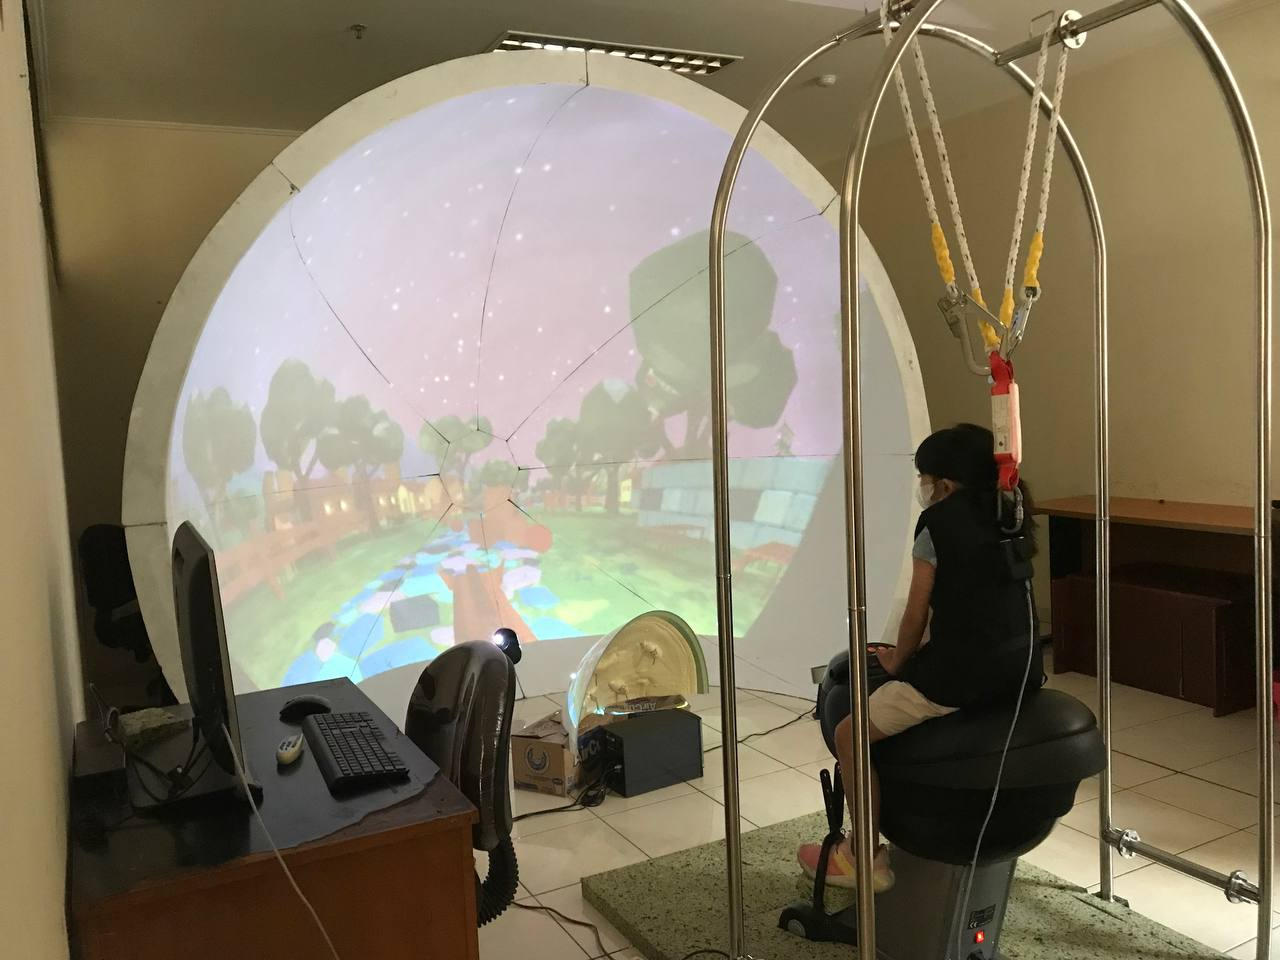
\includegraphics[height=4.5cm]{figs/FotoSystem}}%
		\end{minipage}%
		%\end{adjustwidth}
		\caption
		{%
			(a) System design diagram. (b) Design implementation in use.
			\label{Fig1Horse}%
		}%
\end{figure}

Describe the hardware, highlighting the customization rather than the steps of the procedure. Highlight how it differs/which advantage it offers over pre-existing methods. For example, how could this hardware: be compared to other hardware in terms of cost or ease of use, be used in the development of further designs in a particular area, and so on. \linebreak \linebreak Add 3-5 bulleted points to broadly explain to other researchers how the hardware could be potentially useful to them, for either standard or novel laboratory tasks, inside or outside of the original user community.
\begin{itemize}[noitemsep, topsep=-2pt]
\item Use of the hardware 1
\item Use of the hardware 2
\item Use of the hardware 3
\end{itemize}

\subsection{Dome Design}
As an Immersive Virtual Environment infrastructure, we
build DOME, for several reasons\\

\noindent $D_g$ = eye height in sitting position (cm) for 7-17 years old

\begin{equation}
    F-measure = 2 * \frac{precision * recall}{precision + recall}
    \label{eq4}
\end{equation}

\noindent with:

\noindent $TP$ = True Positive


\section{Design files}

% The  complete  design  files  must  be  either  uploaded  to  an  approved  online  repository,  uploaded  at the  time  of  submission  on  the  online  Editorial  Manager  submission  interface  as  supplementary materials [CAD files, videos,. . . ], or included in the body of the manuscript [e.g.  figures].  The three approved  online  repositories  are  Mendeley  Data,  the  Open  Science  Framework,  and  Zenodo. See repository instructions: https://doi.org/10.5281/zenodo.3346799

% Design files should be in preferred format for making modifications. See OSHWA’s open-source definition for details: https://www.oshwa.org/definition/

for dome design we use, design from paul bourke http://paulbourke.net/dome/iDome/
\textit{The complete design files must be either uploaded to an approved online repository, uploaded at the time of submission on the online \href{https://editorialmanager.com/ohx/}{Editorial Manager} submission interface as supplementary materials [CAD files, videos,\dots], or included in the body of the manuscript [e.g. figures]. The three approved online repositories are \href{https://data.mendeley.com/}{Mendeley Data}, the \href{http://osf.io}{Open Science Framework}, and \href{https://zenodo.org/}{Zenodo}. See repository instructions \href{https://doi.org/10.5281/zenodo.3346799}{here}. Design files should be in preferred format for making modifications. See \href{https://www.oshwa.org/definition/}{OSHWA’s open-source definition} for details.}
\begin{itemize}
\item \textit{CAD files. Authors are encouraged to use free and open source software packages for creating the files. For CAD files, OpenSCAD, FreeCAD, or Blender are encouraged, but if not available source files from proprietary CAD packages such as Autocad or Solidworks and other drawing packages are acceptable.
\item 3D printing. Supplementary files that facilitate the digital replication of the devices are encouraged. For example, STL files for 3-D printing components. We recommend uploading CAD files to the NIH 3D Print Exchange as Custom Labware and providing a link to the location.
\item Electronics. PCB layouts and other electronics design files can be uploaded to the Open Hardware Repository or other repositories.
\item Software and firmware. All software files used in the design and operation of the hardware should be included in the repository. Provide a description of software and firmware and use extensive comments in the code.}
\end{itemize}

%\begin{landscape}
\subsection{Design Files Summary}
% Please include a summary of all design files for your hardware by filling rows of the table below

\tabulinesep=1ex
\begin{tabu} to \linewidth {|X|X|X[1.5,1]|X[1.5,1]|} 
\hline
\textbf{Design file name} & \textbf{File type} & \textbf{Open source license} & \textbf{Location of the file} \\\hline
%Insert design files
\textit{Design file 1} & \textit{e.g. CAD file, figures, videos} & \textit{All designs must be submitted under an open hardware license. Enter the corresponding open source license for the file.} & \textit{Enter a link to the online location or the sentence: ``available with the article'', as appropriate}  \\\hline
\textit{Design file 2} & \dots & \dots & \dots \\\hline
% Design file 3 & File type & License & Link \\\hline
\end{tabu}

% For each design file listed in the summary above, include a short description of the file below (one or two sentences)
\textit{For each design file listed above, include a short description of the file here (one or two sentences)}
%\end{landscape}
\section{Bill of materials}
    
% For a complex Bill of Materials, the complete Bill of Materials (editable spreadsheet file e.g., ODS file type or PDF file) can be uploaded in an open access online location such as the Open Science Framework repository. Include the link here. Alternatively, the Bill of Materials can be uploaded at the time of submission on the online Elsevier submission interface as supplementary material.

% > To make it easy to tell which item in the Bill of Materials corresponds to which component in your design file(s), use matching designators in both places, or otherwise explain the correspondence.

% > For material type, select from: Metal, semi-conductor, ceramic, polymer, biomaterial, organic, inorganic, composite, nanomaterial, semiconductor, non-specific, or other  
\textit{For a complex Bill of Materials, the complete Bill of Materials (editable spreadsheet file e.g., ODS file type or PDF file) can be uploaded in an open access online location such as the Open Science Framework repository. Include the link here. Alternatively, the Bill of Materials can be uploaded at the time of submission on the online Elsevier submission interface as supplementary material.}
\begin{itemize}
\item \textit{To make it easy to tell which item in the Bill of Materials corresponds to which component in your design file(s), use matching designators in both places, or otherwise explain the correspondence.}
\item \textit{For material type, select from: Metal, semi-conductor, ceramic, polymer, biomaterial, organic, inorganic, composite, nanomaterial, semiconductor, non-specific, or other} 
\end{itemize}

%\begin{landscape}
\tabulinesep=1ex
\begin{tabu} to \linewidth {|l|l|l|l|l|l|l|}
\hline
\textbf{Designator} & \textbf{Component} & \textbf{Number} & \textbf{Cost per unit - USD} & \textbf{Total cost - USD} & \textbf{Source of materials} & \textbf{Material type} \\\hline

%Insert items here
\textit{Designator 1} & \textit{Name of Component 1} & \textit{Number of units} & \textit{Cost per unit} & \textit{Total cost} & \textit{Source} & \textit{Material type} \\\hline
\textit{Designator 2} & \dots & \dots & \dots & \dots & \dots & \dots \\\hline
% Designator 3 & Name of Component 2 & Number of units & Cost per unit & Total cost & Source of materials & Material type \\\hline
\end{tabu}
%\end{landscape}
\section{Build instructions}
    
%Provide detailed, step by step instructions for the construction of the reported hardware include all necessary information for reproducing the submitted hardware.
% > Explain and, when possible, characterize design decisions. Including design alternatives if they exist. 
% > Use visual instructions such as schematics, images, and videos. 
% > Clearly reference design files and component parts described in the Design File Summary and Bill of Materials. 
% >Highlight potential safety concerns that may arise

\textit{Provide detailed, step by step instructions for the construction of the reported hardware
 include all necessary information for reproducing the submitted hardware.
\begin{itemize}
\item Explain and, when possible, characterize design decisions. Including design alternatives if they exist. 
\item Use visual instructions such as schematics, images, and videos. 
\item Clearly reference design files and component parts described in the Design File Summary and Bill of Materials. 
\item Highlight potential safety concerns that may arise
\end{itemize}}

\section{Operation instructions}
    
%Provide detailed instructions for the safe and proper operation of the hardware. 
%> Step-by-step operational instructions for operating the hardware. 
%> Use visual instructions as necessary. 
%> Highlight potential safety hazards.

\textit{Provide detailed instructions for the safe and proper operation of the hardware. 
\begin{itemize}
\item Step-by-step operational instructions for operating the hardware. 
\item Use visual instructions as necessary. 
\item Highlight potential safety hazards.
\end{itemize}}
\section{Validation and characterization}
    
%Demonstrate the operation of the hardware and characterize its performance over relevant critical metrics
%> Demonstrate the use of the hardware for a relevant use case. 
%> If possible, characterize performance of the hardware over operational parameters. 
%> Create a bulleted list that describes the capabilities (and limitations) of the hardware. For example consider descriptions of load, operation time, spin speed, coefficient of variation, accuracy, precision and etc. 

\textit{Demonstrate the operation of the hardware and characterize its performance over relevant critical metrics
\begin{itemize}
\item Demonstrate the use of the hardware for a relevant use case. 
\item If possible, characterize performance of the hardware over operational parameters. 
\item Create a bulleted list that describes the capabilities (and limitations) of the hardware. For example consider descriptions of load, operation time, spin speed, coefficient of variation, accuracy, precision and etc. 
\end{itemize}}


% \newpage
\section{Acknowledgements}
This research works was funded by Lembaga Pengembangan Inovasi dan Kewirausahaan, Institut Teknologi Bandung (LPIK ITB) under the grant "Program Penguatan Inovasi 2021" number 289L/IT1.A/SK-KP/2021 and School of Electrical Engineering and Informatics, Institut Teknologi Bandung, under the grant "Program Penelitian, Pengabdian kepada Masyarakat dan Inovasi, Institut Teknologi Bandung, 2021 (P2MI-ITB 2021)" number 917/IT1.C12/KP/2021.

The article processing charge (APC) was funded by School of Electrical Engineering, Telkom University.
\section{Declaration of interest}
% a statement must be included even if there is no conflict of interest
% All authors must disclose any financial and personal relationships with other people or organizations that could inappropriately influence (bias) their work. Examples of potential conflicts of interest include employment, consultancies, stock ownership, honoraria, paid expert testimony, patent applications/registrations, and grants or other funding. Authors must disclose any interests in a summary declaration of interest statement in the manuscript file. If there are no interests to declare then please state this: 'Declarations of interest: none'. This summary statement will be ultimately published if the article is accepted. More information.}

The authors declare that no known personal relationships and/or financial interests that could have influenced the work reported in this paper.
\section{Human and animal rights}
%> If the work involves the use of human subjects, the author should ensure that the work described has been carried out in accordance with the appropriate ethical guidelines.
%> If the work involves the use of human subjects, the author should ensure that the work described has been carried out in accordance with The Code of Ethics of the World Medical Association (Declaration of Helsinki) for experiments involving humans; Uniform Requirements for manuscripts submitted to Biomedical journals. Authors should include a statement in the manuscript that informed consent was obtained for experimentation with human subjects. The privacy rights of human subjects must always be observed.
%> All animal experiments should comply with the ARRIVE guidelines and should be carried out in accordance with the U.K. Animals (Scientific Procedures) Act, 1986 and associated guidelines, EU Directive 2010/63/EU for animal experiments, or the National Institutes of Health guide for the care and use of Laboratory animals (NIH Publications No. 8023, revised 1978) and the authors should clearly indicate in the manuscript that such guidelines have been followed

The author declare that the work reported has been carried out in accordance with The Code of Ethics of the World Medical Association (Declaration of Helsinki). Informed consent was obtained from all subjects involved in the study and their privacy rights is preserved.

\end{flushleft}

\section*{References} 
%> Include at least one reference, to the original publication of the hardware you customized.
%> Include other references as required. Include references to put your device in context in the literature. For more information on the reference format in HardwareX please see the Guide for Authors at: https://www.elsevier.com/journals/hardwarex/2468-0672/guide-for-authors

\textit{\begin{itemize}
\item Include at least one reference, to the original publication of the hardware you customized.
\item Include other references as required. Include references to put your device in context in the literature. For more information on the reference format in HardwareX please see the Guide for Authors at: https://www.elsevier.com/journals/hardwarex/2468-0672/guide-for-authors
\end{itemize}}

% menampilkan referensi %%%%%%%%%%%%%%%%%%%%%%%%%%%%%%%%%%%%
%\printbibliography
\bibliographystyle{ieeetr}
\bibliography{references}

\end{document}

%> Author manuscript checklist
%> ●	HardwareX is a journal dedicated to the exhaustive and fully open source communication of advances in scientific infrastructure. Upon submission the author declares that all information necessary to reproduce the subject of the submission (e.g. bill of materials, build instructions, calibration procedures, source files, code, and safety considerations) is communicated in full and is accessible for use under an open source license. 
%> ●	Is the subject of the submission under an open source license? Are design files in the preferred format for making modifications? As defined by the Open Source Hardware definition. 
%> ●	Can the hardware be reproduced with the details provided in the submission?
%> ●	Are all relevant design files available on Mendeley Data, the Open Science Framework, or Zenodo repositories, described in the Summary of Design Files document, and clearly documented? (e.g. descriptive file names, commented code, labeled images, etc.) 
%>      ○	If in the Open Science Framework, the repository has be registered? Instructions
%>      ○	If in Zenodo, the repository is open access and is published? Instructions
%>      ○	If in Mendeley Data, the repository is published or the sharable link was included in the additional information of the Editorial Submission interface? Instructions
%> ●	Are visual instructions used when necessary?
%> ●	Is the utility of the hardware to the scientific community? Has a specific scientific application been demonstrated using the hardware?
%> ●	Is the performance of the hardware adequately demonstrated and characterized?
%> ●	Are all potential safety concerns addressed?
%> ●	For more information on the article template consult the Guide to Authors.}
